\documentclass[letterpaper,11pt]{article}
\usepackage[spanish, es-tabla]{babel}
\usepackage[utf8]{inputenc}
\usepackage{graphicx,amsmath,amssymb,ragged2e,tabularx,multirow,natbib,bibentry,graphics,color,float}
\usepackage[bookmarks, colorlinks, breaklinks]{hyperref}  
\hypersetup{linkcolor=red,citecolor=red,filecolor=black,urlcolor=green}
\usepackage{listingsutf8}



	\title{R inicial}
%\subtitle{Presentación del curso}
\author{Valentín Vergara Hidd}
%\institute[UdeC]{Universidad de Concepción}
\date{\today}
%\logo{udec}

\oddsidemargin=0cm
\textwidth=16cm

%\setbeamertemplate{navigation symbols}{}
%\usetheme{Madrid}
%\usecolortheme{albatross}
%\usecolortheme[named=Black]{structure}\lstset{% general command to set parameter(s)

%\usefonttheme[onlymath]{serif}
%\justifying

%\usebackgroundtemplate{\scalebox{0.6}{\includegraphics[width=\paperwidth]{ko.eps}}}
%\pgfdeclareimage[height=1.2cm, width=1cm]{logo}{udec}
%\logo{\pgfuseimage{logo}}



\begin{document}
\lstset{% general command to set parameter(s)
	language=R,
	basicstyle=\scriptsize\ttfamily, % print whole listing small
	keywordstyle=\color{cyan},
	framexleftmargin=-2pt,
	%backgroundcolor=\color{gray!10},
	frame=single,
	tabsize=2,
	%rulecolor=\color{black!30},
	title=\lstname,
	escapeinside={\%*}{*)},
	breaklines=true,
	breakatwhitespace=true,
	framextopmargin=-5pt,
	framexbottommargin=-5pt,
	extendedchars=false,
	inputencoding=utf8,
	literate={á}{{\'{a}}}1, 
	literate={é}{{\'{e}}}1,	
	literate={ó}{{\'{o}}}1,
	literate={ú}{{\'{u}}}1,
	literate={ñ}{{\~{n}}}1, 
	literate={í}{{\'{i}}}1
}

\maketitle

%\renewcommand{\listtablename}{Índice de tablas} 
%\renewcommand{\tablename}{Tabla} 

La intención de este documento es ser una primera aproximación al uso del \emph{lenguaje} R. Como tal, su intención no es comenzar a trabajar en funciones ni en estructuras más avanzadas, sino que simplemente familiarizarse con la instalación, espacios de trabajo, uso de paquetes y funcionamiento de objetos. 

Como requisito para el trabajo con este documento, se requiere tener instalado R\footnote{Software libre que se puede obtener en \href{https://www.r-project.org/}{este sitio}} y aunque no es necesario, sugiero complementarlo con una GUI\footnote{\emph{Graphical User Interface}}, de las cuales recomiendo R Studio\footnote{Software comercial, con una de sus licencias de uso gratuito, que se puede encontrar en \href{https://www.rstudio.com/}{este sitio}}.

\section{Contexto}
R es una implementación del lenguaje de programación \href{http://ect.bell-labs.com/sl/S/}{S}, que siguió su propio camino de desarrollo a partir de 1992 en la Universidad de Auckland, Nueva Zelanda. Su desarrollo estuvo a cargo de Ross Ihaka y Robert Gentleman (de ahí el nombre R). La primera versión estable (beta) se lanzó en 2000, momento desde el que ha adquirido cada vez más popularidad en el mundo académico.

Como se observa en la imagen a continuación, el uso de R ha ido en constante aumento desde su primera versión estable. Se atribuye esta creciente popularidad en que es \emph{software libre}, pero que además utiliza un lenguaje para programar funciones que es amigable con quienes no son programadores. Esto ha posibilitado que muchos académicos dedicados a la estadística, hayan creado \emph{paquetes} para implementar algoritmos nuevos en R. A todo lo anterior se suman sus capacidades profesionales para gráficos, que generalmente es un punto débil de otros software estadísticos. 

\begin{figure}[H]
\centering
\scalebox{0.9}{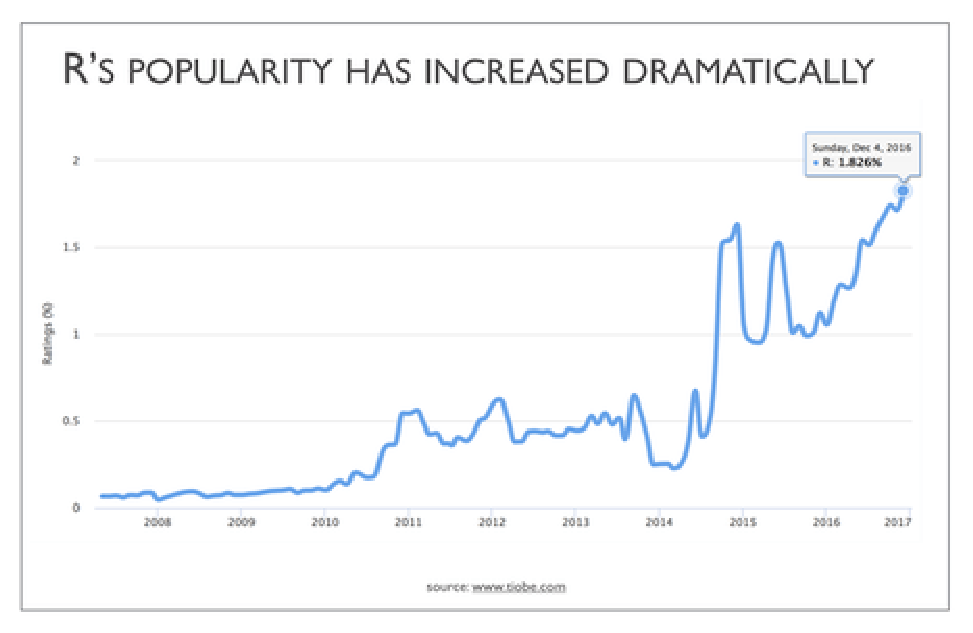
\includegraphics{3_01}}
\caption{Uso de R en \emph{data science} desde el año 2000}
\end{figure}

\section{La consola como punto de partida}

R trabaja con una consola, que no es otra cosa que un terminal de texto donde se escriben las instrucciones y donde se muestran algunos resultados. Al ejecutar R (no R Studio, eso lo veremos más adelante), desde cualquier sistema operativo, deberían visualizar lo siguiente:

\begin{figure}[H]
	\centering
	\scalebox{0.55}{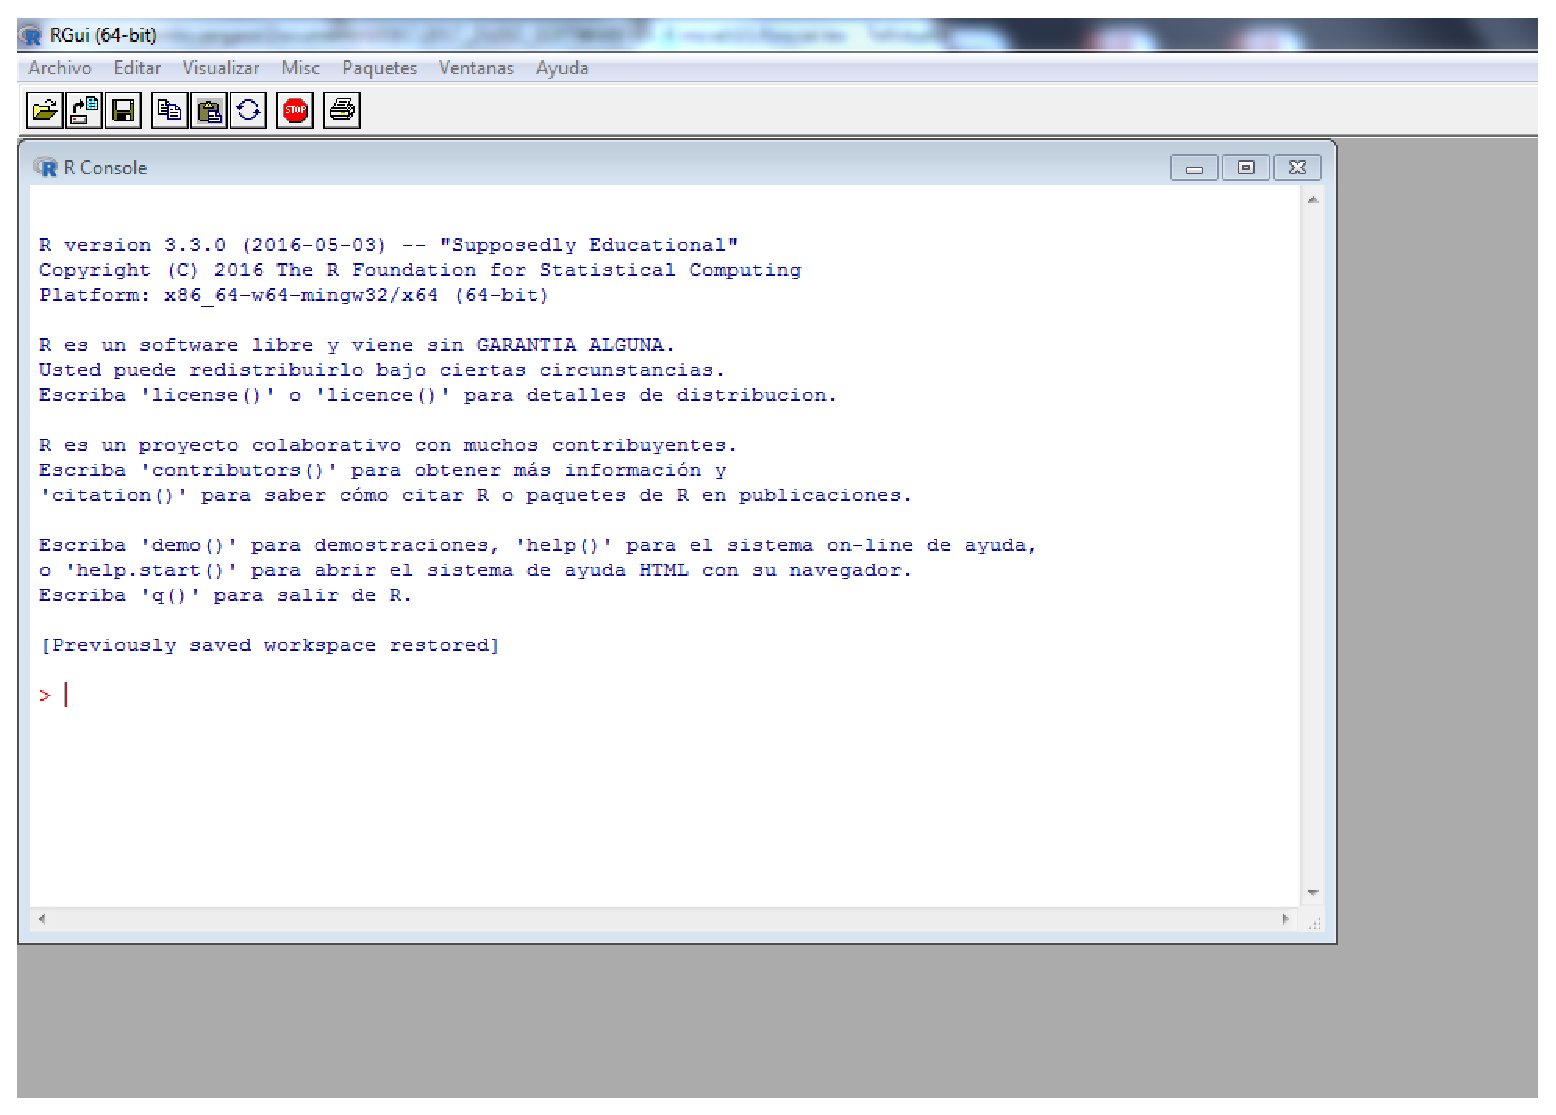
\includegraphics{3_02}}
	\caption{Vista inicial de R, en Windows}
\end{figure}

Donde se encuentra el cursor, se puede comenzar a escribir, con la consideración que para ejecutar una instrucción, se debe presionar la tecla Enter.

\subsection{R como una calculadora}

R funciona \emph{como} una calculadora, principalmente debido a que al ingresar expresiones en la consola, obtenemos su resultado, si eso es posible. Por ejemplo, si nos interesa una suma entre dos números (6 y 19), ingresamos

\begin{lstlisting}
> 6 + 19
[1] 25
\end{lstlisting}

El signo \emph{mayor que} se conoce como el {\bf prompt}, lo que significa que al aparecer ese signo, la consola de R está lista pàra recibir más instrucciones. Podrán notar que en el ejemplo anterior se utilizó el operador $+$. De la misma forma, existen otros operadores que se pueden utilizar, algunos de los cuales se encuentran en la tabla a continuación.

\begin{table}[H]
\centering
\caption{Algunos operadores numéricos en R. Se asume que $x$ y $y$ son números.}
\begin{tabular}{cll}
	\multicolumn{3}{c}{}\\
\hline \hline
Operador	& Definición & Ejemplo\\
\hline
+ & Adición & {\ttfamily x + y}\\
- & Sustracción & {\ttfamily x - y}\\
* & Multiplicación & {\ttfamily x*y}\\
/ & División & {\ttfamily x/y}\\
\textasciicircum & Potencia & {\ttfamily x\textasciicircum y} \\
log() & Logaritmo natural & {\ttfamily log(x)}\\
log10() & Logaritmo base 10 & {\ttfamily log10(x)}\\
log(x,y) & Logaritmo base $y$ & {\ttfamily log(x,y)}\\
sqrt() & Raíz Cuadrada & {\ttfamily sqrt(x)}\\

\hline 
\end{tabular}
\end{table}

Es importante señalar que R considera las expresiones en un sentido algebraico, por lo que se debe cuidar el uso de paréntesis donde corresponda. Si sabemos, por ejemplo, que 
\begin{equation*}
23 + 7 + 14 \div 2 \neq (23 + 7 + 14)\div 2
\end{equation*}

Lo podemos probar en R.

\begin{lstlisting}
> 23 + 7 + 14 / 2
[1] 37
> (23 + 7 + 14) / 2
[1] 22
\end{lstlisting}

Como nota adicional, considere que el 1 que aparece entre corchetes indica que el resultado de la operación solicitada es un vector cuyo primer elemento se \emph{imprime} en la pantalla. Además, existe la posibilidad de obtener un error, si es que lo que se entrega como valor entre los operadores no corresponde a un número ni a un objeto previamente asignado en R.

\begin{lstlisting}
> x + y
Error: object 'x' not found
\end{lstlisting}

Al intentar ingresar la instrucción anterior en la consola, se obtiene un error, al comprobar que $x$ no es un número; ni tampoco un objeto en la memoria, por lo que el proceso se detiene sin siquiera alcanzar a evaluar $y$.

También se debe considerar que se pueden combinar distintos operadores, por ejemplo.

\begin{lstlisting}
> log(500*2, sqrt(100))
[1] 3
\end{lstlisting}

\section{Objetos}

Como ya se mencionó, si intentamos sumar $x$ y $y$ sin que estos sean \emph{objetos} previamente guardados en la memoria de la sesión abierta de R, vamos a obtener un error. La solución, es asignar valores a estas letras. El operador fundamental para esto es {\ttfamily <-} (El signo \emph{menor que} seguido de un guión). Lo que sea que quede a la izquierda de este operador, será el objeto; y lo que sea que quede a la derecha, va a ser el contenido de ese objeto.

Lo más simple que podemos asignar a un objeto es un valor numérico. Es decir, una constante:

\begin{lstlisting}
> x<-10
> y<-17
> x + y
[1] 27
\end{lstlisting}

También podemos usar algunas expresiones ya creadas dentro de otras. Por ejemplo:

\begin{lstlisting}
> x<-27/3
> y<-log(x)
> z<-exp(y)
> z
[1] 9
\end{lstlisting}

Aprovechando las propiedades de $e$ y de los logaritmos naturales, probamos que se pueden incluir valores de objetos en otros objetos.


\end{document}